\section{PRESENTACION DEL ESPACIO DE TRABAJO} 

	\begin{center}
	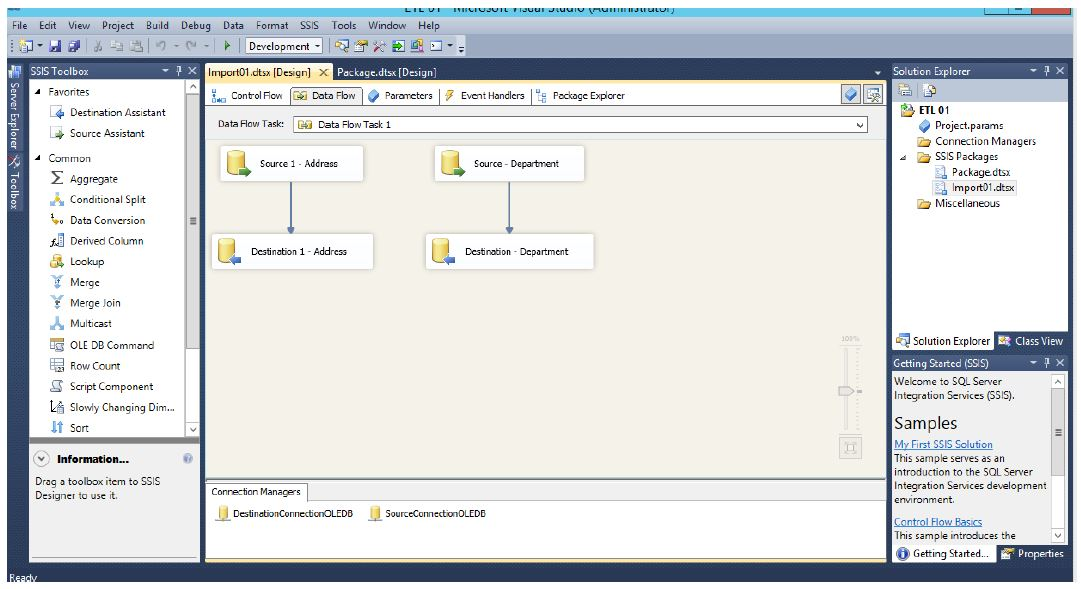
\includegraphics[width=15cm]{./Imagenes/10}
	\end{center}	

- MI PRIMER PAQUETE, Muestra la cantidad de Registros de una Tabla\\
- File - \textgreater NewProject - \textgreater

	\begin{center}
	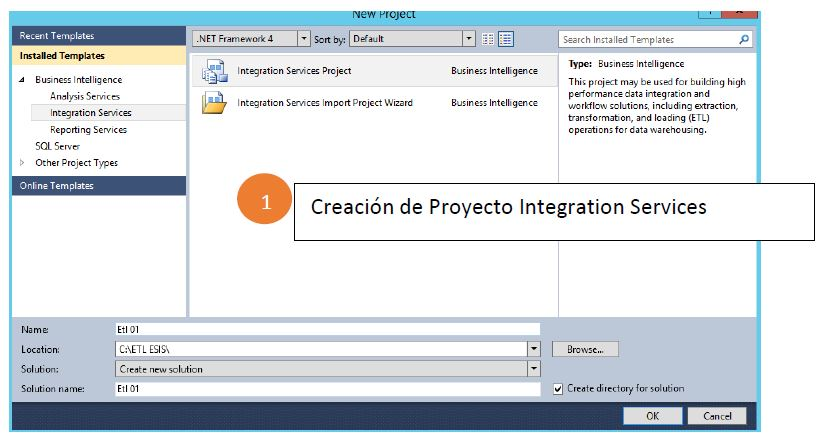
\includegraphics[width=15cm]{./Imagenes/11}
	\end{center}	

2. Creacion una conexión OLEDB para la base de datos Adventure Work.

	\begin{center}
	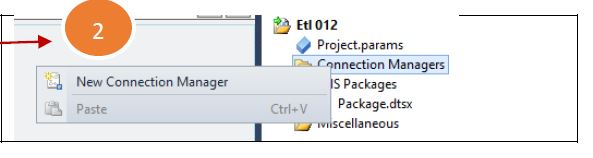
\includegraphics[width=12cm]{./Imagenes/111}
	\end{center}	

- Selección de OLEDB como Driver de Conexión BD

	\begin{center}
	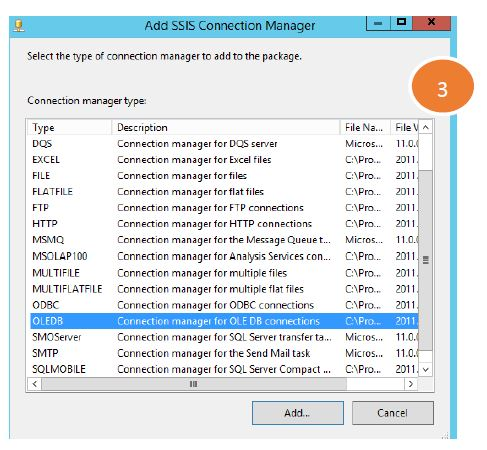
\includegraphics[width=13cm]{./Imagenes/12}
	\end{center}	

- Configuración de Conexión.

	\begin{center}
	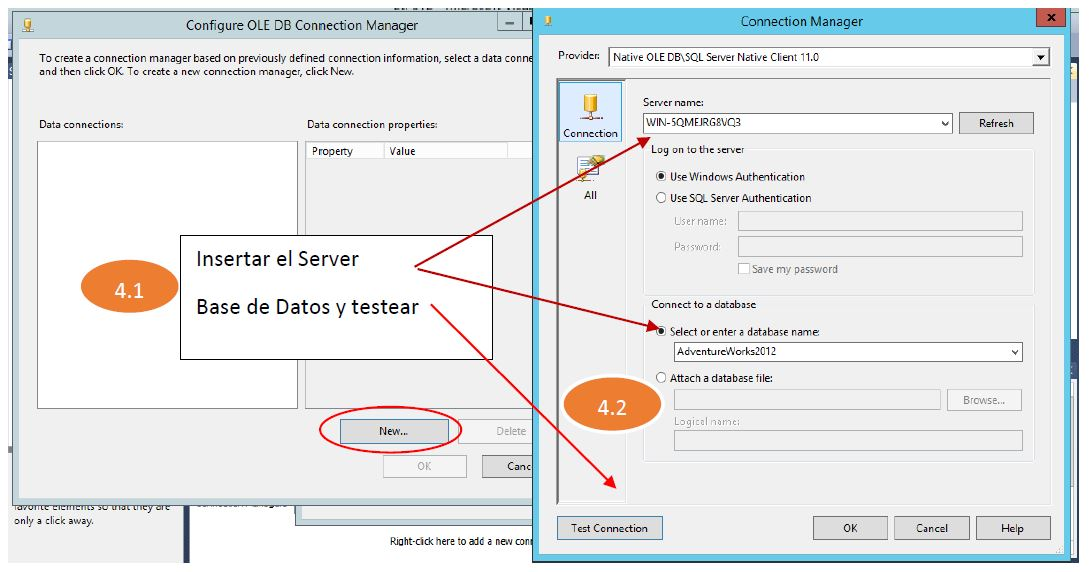
\includegraphics[width=17cm]{./Imagenes/13}
	\end{center}	

- Resultado de la Configuración.

	\begin{center}
	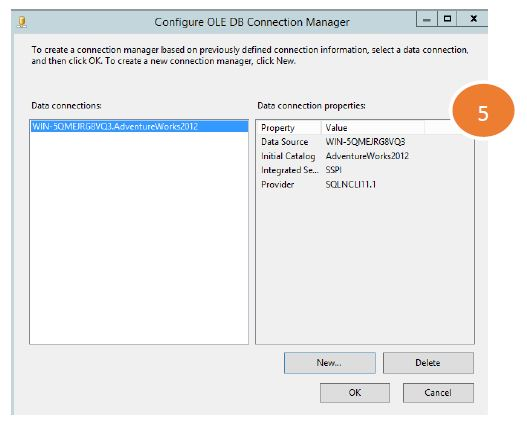
\includegraphics[width=14cm]{./Imagenes/14}
	\end{center}	

\begin{itemize}
    \item \textbf{Insertar: Execute SQL Task y Script Task}

	\begin{center}
	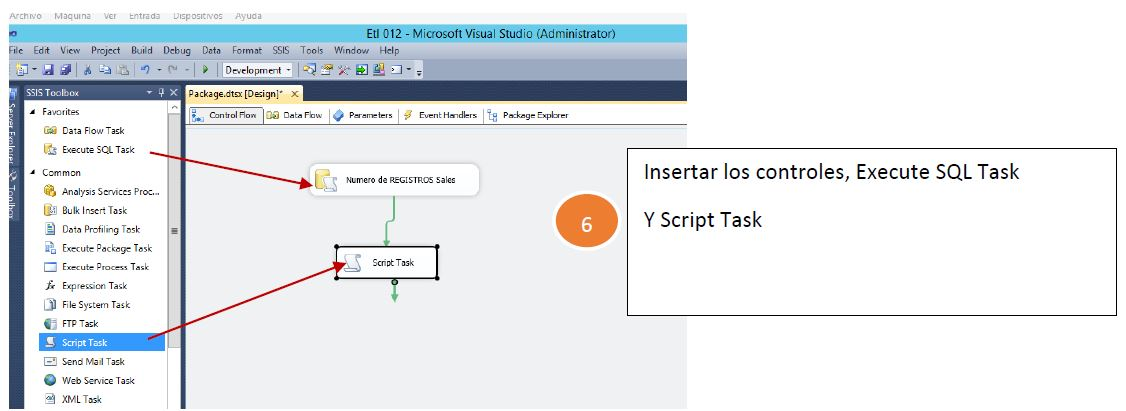
\includegraphics[width=17cm]{./Imagenes/15}
	\end{center}	

	\begin{center}
	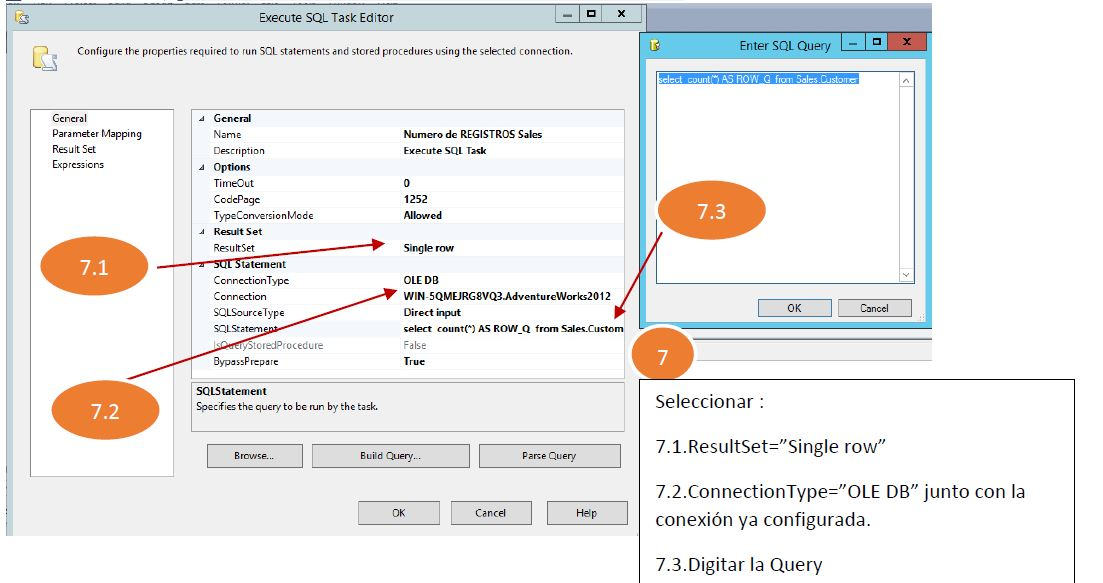
\includegraphics[width=17cm]{./Imagenes/16}
	\end{center}	

- Crear la Variable:

	\begin{center}
	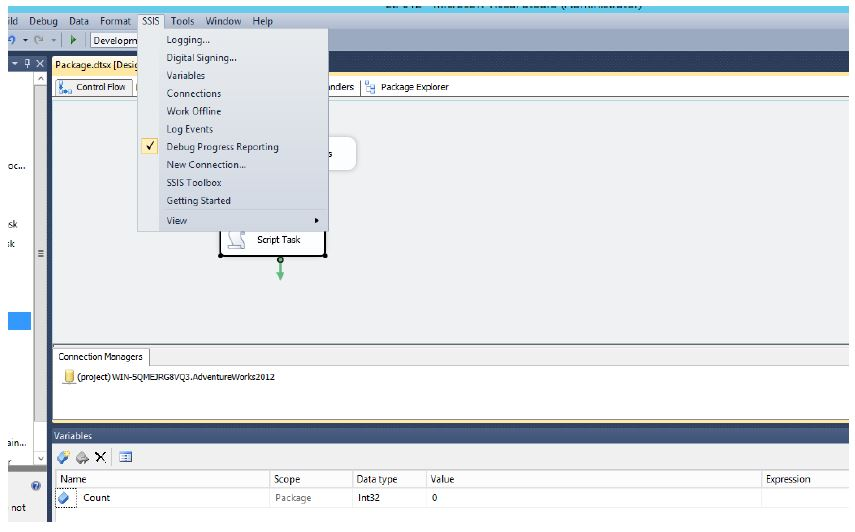
\includegraphics[width=15cm]{./Imagenes/17}
	\end{center}	

- Asignar la variable en “Numero de Registros Sales”.

	\begin{center}
	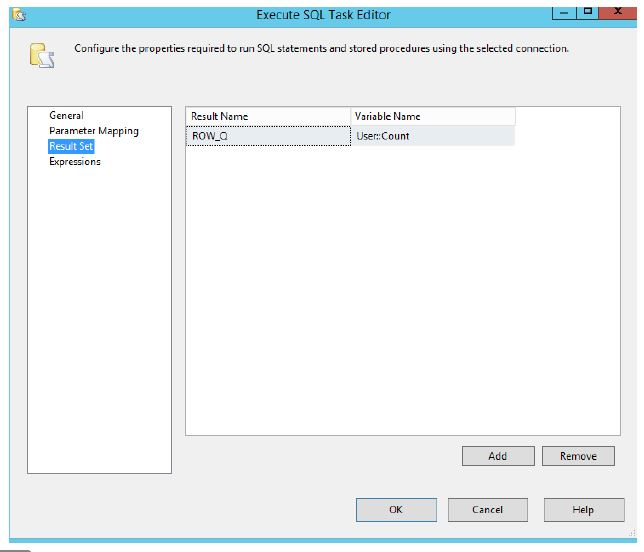
\includegraphics[width=13cm]{./Imagenes/18}
	\end{center}	

    \item \textbf{EDITAR COMPONENTE “Script Task Editor”}

	\begin{center}
	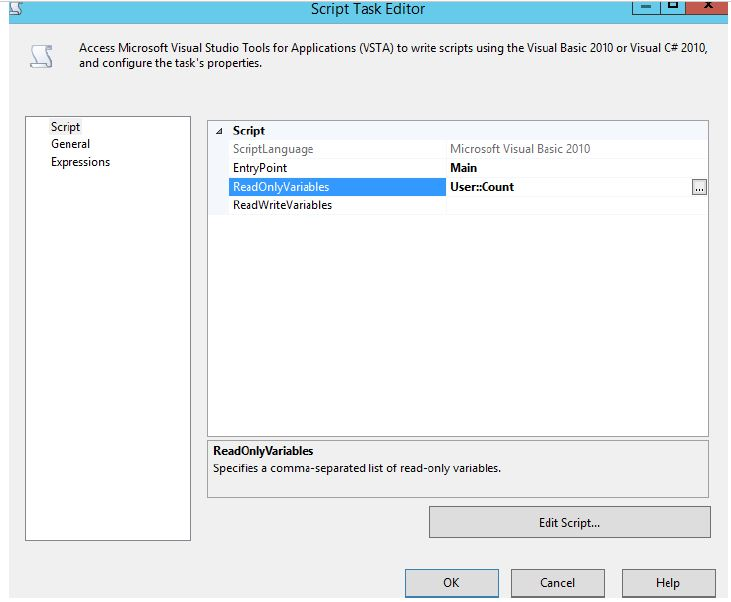
\includegraphics[width=13cm]{./Imagenes/19}
	\end{center}	

- Insertar este código “MsgBox(Dts.Variables(0).Value, MsgBoxStyle.Information)”

	\begin{center}
	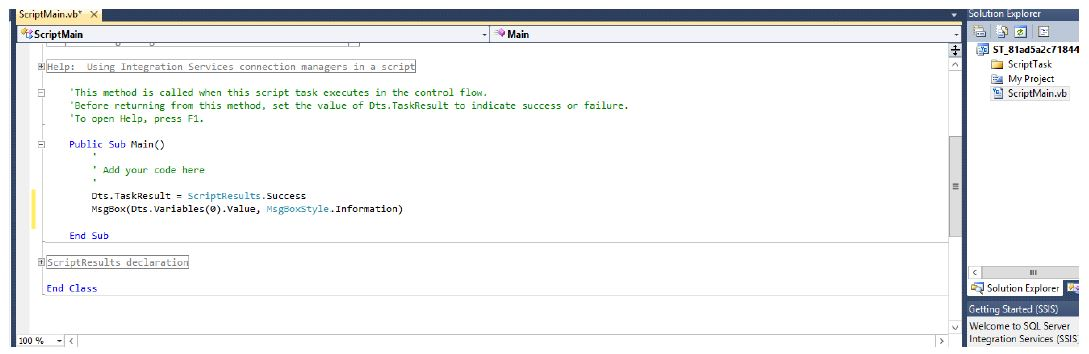
\includegraphics[width=17cm]{./Imagenes/20}
	\end{center}	

- Guardamos el proyecto y EJECUTAMOS Y LISTO.

	\begin{center}
	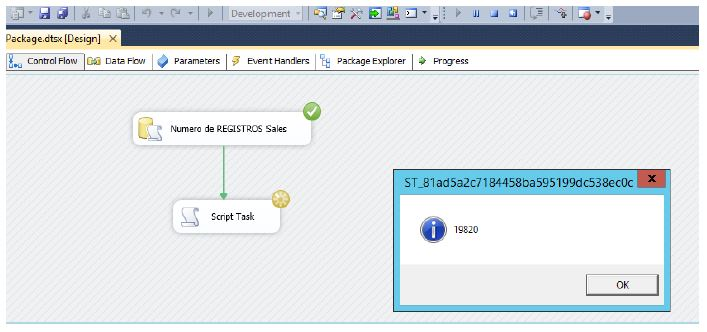
\includegraphics[width=15cm]{./Imagenes/21}
	\end{center}	
\end{itemize}